
\subsection{Scaling Options}

\begin{pgfplotskey}{width=\marg{dimen}}
Sets the width of the final picture to \marg{dimen}. If no |height| is specified, scaling will respect aspect ratios.

\paragraph{Remarks:} 
\begin{itemize}
	\item The scaling only affects the width of one unit in $x$-direction or the height for one unit in $y$-direction. Axis labels and tick labels won't be resized, but their size is used to determine the axis scaling.

	\item You can use the |scale=|\marg{number} option,
\begin{codeexample}[code only]
\begin{tikzpicture}[scale=2]
\begin{axis}
...
\end{axis}
\end{tikzpicture}
\end{codeexample}
	to scale the complete picture.

	\item The \Tikz-options |x| and |y| which set the unit dimensions in $x$ and $y$ directions can be specified as arguments to |\begin{axis}[x=1.5cm,y=2cm]| if needed (see below). These settings override the |width| and |height| options.

	\item You can also force a fixed width/height of the axis (without looking at labels) with
\begin{codeexample}[code only]
\begin{tikzpicture}
\begin{axis}[width=5cm,scale only axis]
	...
\end{axis}
\end{tikzpicture}
\end{codeexample}

	\item Please note that up to the writing of this manual, \PGFPlots\ only estimates the size needed for axis- and tick labels. It does not include legends which have been placed outside of the axis\footnote{I.e. the `\texttt{width}' option will not work as expected, but the bounding box is still ok.}. This may be fixed in future versions.

	Use the |x=|\marg{dimension}, |y=|\marg{dimension} and |scale only axis| options if the scaling happens to be wrong.
\end{itemize}
\end{pgfplotskey}

\begin{pgfplotskey}{height=\marg{dimen}}
	See |width|.
\end{pgfplotskey}

\begin{pgfplotskey}{scale only axis=\mchoice{true,false} (initially false)}
If |scale only axis| is enabled, label, tick and legend dimensions won't influence the size of the axis rectangle, that means |width| and |height| apply only to the axis rectangle

If |scale only axis=false| (the default), \PGFPlots\ will try to produce the desired width \emph{including} labels, titles and ticks.
\end{pgfplotskey}

\begin{pgfplotsxykeylist}{
	\x=\marg{dimen},
	\x={\{(\meta{x},\meta{y})\}}}
Sets the unit vectors for $x$ (or $y$). Every logical plot coordinate $(x,y)$ is drawn at the position
\[ x \cdot \begin{bmatrix} e_{xx} \\ e_{xy} \end{bmatrix} + y \cdot \begin{bmatrix} e_{yx} \\ e_{yy} \end{bmatrix}. \]
The unit vectors $e_x$ and $e_y$ determine the paper position in the current (always two dimensional) image.

The key |x=|\marg{dimen} simply sets $e_x = (\meta{dimen},0)^T $ while |y=|\marg{dimen} sets $e_y = (0,\meta{dimen})^T$.
Here, \marg{dimen} is any \TeX\ size like |1mm|, |2cm| or |5pt|. It is allowed to specify a negative \marg{dimen}.
\begin{codeexample}[]
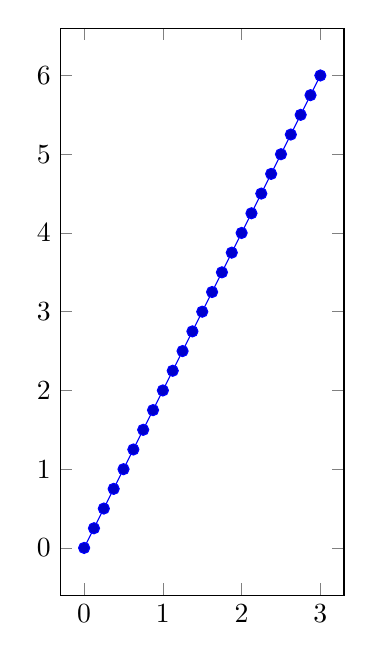
\begin{tikzpicture}
\begin{axis}[x=1cm,y=1cm]
\addplot expression[domain=0:3] {2*x};
\end{axis}
\end{tikzpicture}
\end{codeexample}

\begin{codeexample}[]
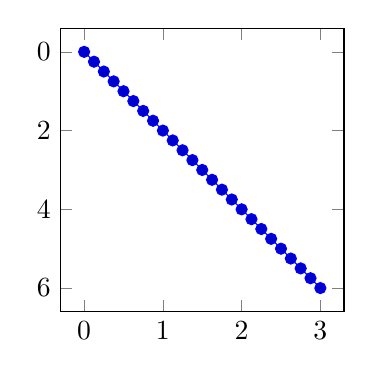
\begin{tikzpicture}
\begin{axis}[x=1cm,y=-0.5cm]
\addplot expression[domain=0:3] {2*x};
\end{axis}
\end{tikzpicture}
\end{codeexample}

The second syntax, |x={(|\meta{x}|,|\meta{y}|)}| sets $e_x = (\meta{x},\meta{y})^T$ explicitly\footnote{Please note that you need extra curly braces around the vector. Otherwise, the comma will be interpreted as separator for the next key-value pair.}; the corresponding |y| key works similarly. This allows to define skewed or rotated axes.

\begin{codeexample}[]
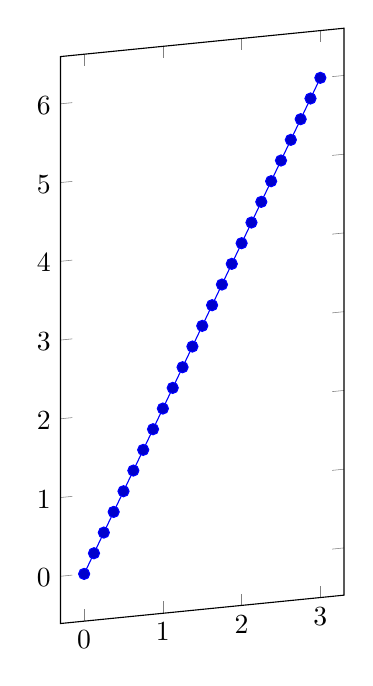
\begin{tikzpicture}
\begin{axis}[x={(1cm,0.1cm)},y=1cm]
\addplot expression[domain=0:3] {2*x};
\end{axis}
\end{tikzpicture}
\end{codeexample}

\begin{codeexample}[]
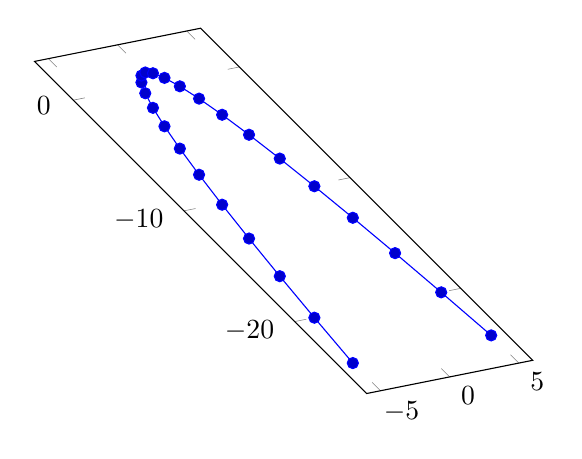
\begin{tikzpicture}
\begin{axis}[
		x={(5pt,1pt)},
		y={(-4pt,4pt)}]
\addplot {1-x^2};
\end{axis}
\end{tikzpicture}
\end{codeexample}

	Setting $x$ explicitly overrides the |width| option. Setting $y$ explicitly overrides the |height| option.

	Setting |x| and/or |y| for logarithmic axis will set the dimension used for $1 \cdot e \approx 2.71828$.

	Please note that it is \emph{not} possible to specify |x| as argument to |tikzpicture|. The option 
\begin{codeexample}[code only]
\begin{tikzpicture}[x=1.5cm]
\begin{axis}
	...
\end{axis}
\end{tikzpicture}
\end{codeexample}
	won't have any effect because an axis rescales its coordinates (see the |width| option).

\paragraph{Limitations:} Unfortunately, skewed axes are \textbf{not available for bar plots}.
\index{Errors!Skewed axes and bar plots}%
\index{Bar Plots!Skewed axes problems}%
Furthermore, support for custom vectors in 3D plots is currently \textbf{experimental} and may not work at all, sorry.
\end{pgfplotsxykeylist}

\begin{pgfplotsxykey}{\x mode=\mchoice{normal,linear,log} (initially normal)}
	Allows to choose between linear (=normal) or logarithmic axis scaling or logplots for each $x,y,z$-combination.

	Logarithmic plots use the current setting of |log basis x| and its variants to determine the basis (default is $e$).
	% FIXME : replicated in pgfplots.reference.specifyrange.tex
\end{pgfplotsxykey}

{\def\pgfmanualpdflabel#1#2{}
\begin{pgfplotsxykey}{\x\ dir=\mchoice{normal,reverse} (initially normal)}
	Allows to revert axis directions such that values are given in decreasing order.

	This key is documented in all detail on page~\pageref{key:pgfplots:xydir}.
\end{pgfplotsxykey}
}

\begin{pgfplotskey}{axis equal=\marg{true,false} (initially false)}
	Each unit vector is set to the same length while the axis dimensions stay constant. Afterwards, the size ratios for each unit in $x$ and $y$ will be the same.
	
	Axis limits will be enlarge to compensate for the scaling effect.
\begin{codeexample}[]
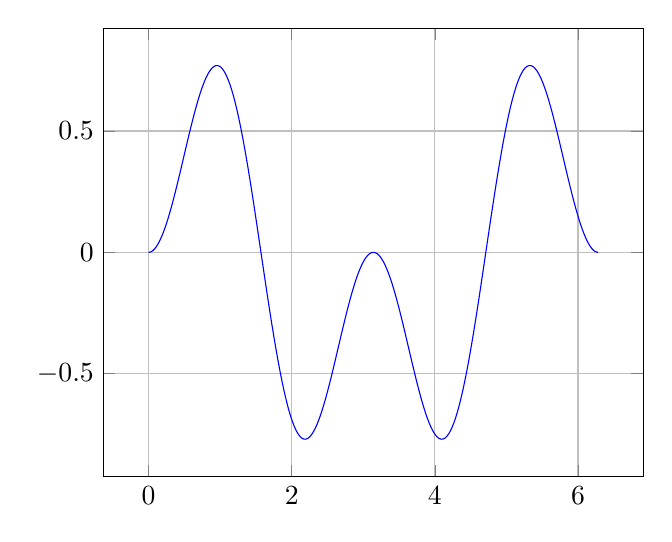
\begin{tikzpicture}
	\begin{axis}[axis equal=false,grid=major]
		\addplot[blue] expression[domain=0:2*pi,samples=300] {sin(deg(x))*sin(2*deg(x))};
	\end{axis}
\end{tikzpicture}
\hspace{1cm}
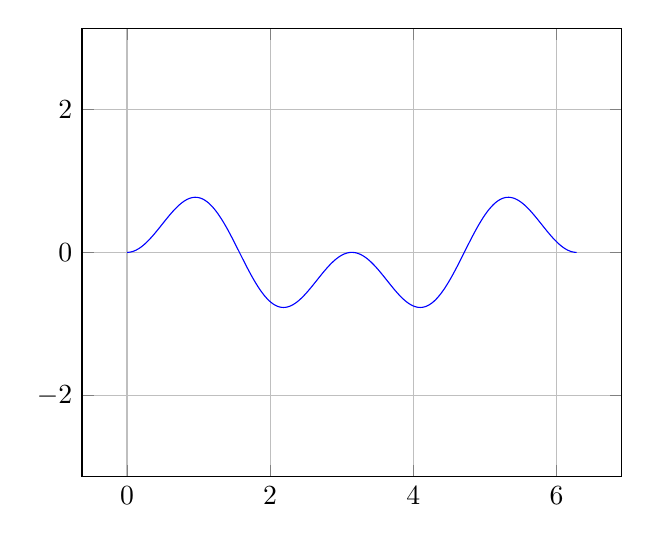
\begin{tikzpicture}
	\begin{axis}[axis equal=true,grid=major]
		\addplot[blue] expression[domain=0:2*pi,samples=300] {sin(deg(x))*sin(2*deg(x))};
	\end{axis}
\end{tikzpicture}
\end{codeexample}
	
\begin{codeexample}[]
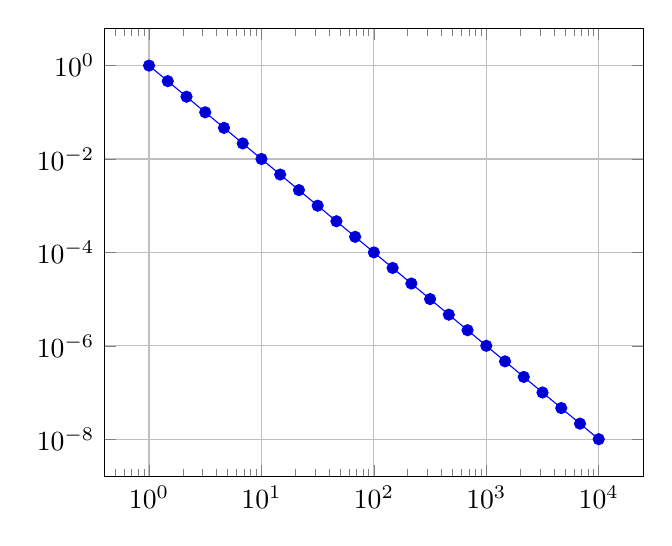
\begin{tikzpicture}
	\begin{loglogaxis}[axis equal=false,grid=major]
		\addplot expression[domain=1:10000] {x^-2};
	\end{loglogaxis}
\end{tikzpicture}
\hspace{1cm}
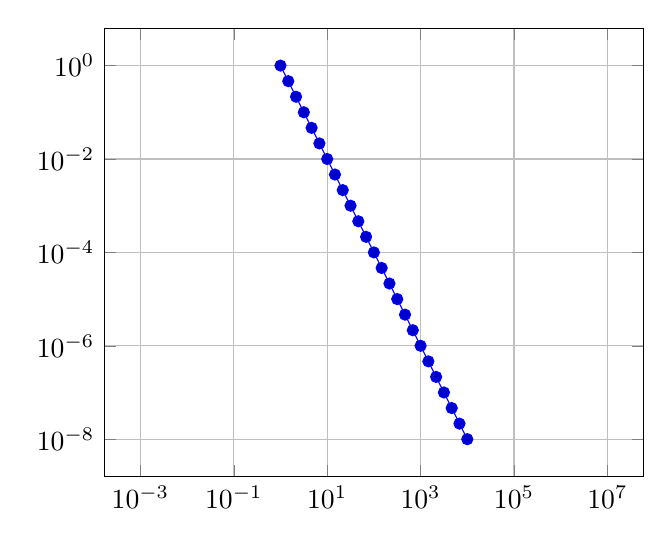
\begin{tikzpicture}
	\begin{loglogaxis}[axis equal=true,grid=major]
		\addplot expression[domain=1:10000] {x^-2};
	\end{loglogaxis}
\end{tikzpicture}
\end{codeexample}
\end{pgfplotskey}

\begin{pgfplotskey}{axis equal image=\marg{true,false} (initially false)}
	Similar to |axis equal|, but the axis limits will stay constant as well (leading to smaller images).
\begin{codeexample}[]
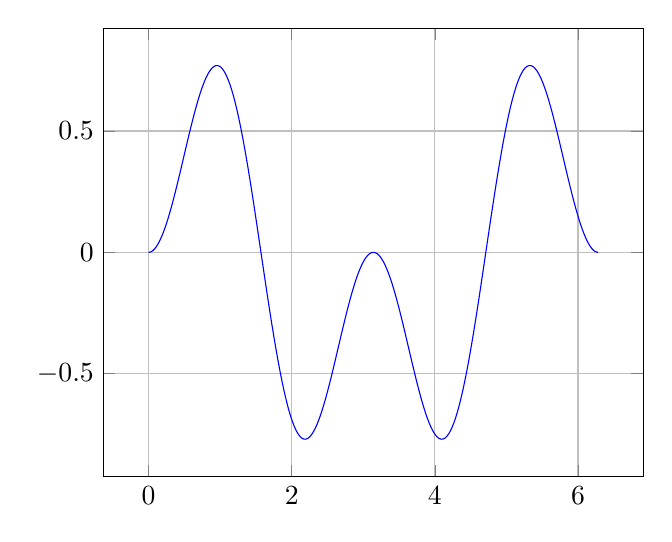
\begin{tikzpicture}
	\begin{axis}[axis equal image=false,grid=major]
		\addplot[blue] expression[domain=0:2*pi,samples=300] {sin(deg(x))*sin(2*deg(x))};
	\end{axis}
\end{tikzpicture}
\hspace{1cm}
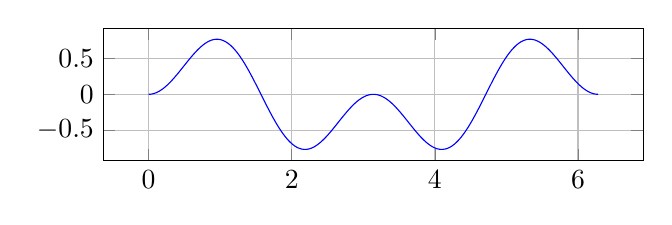
\begin{tikzpicture}
	\begin{axis}[axis equal image=true,grid=major]
		\addplot[blue] expression[domain=0:2*pi,samples=300] {sin(deg(x))*sin(2*deg(x))};
	\end{axis}
\end{tikzpicture}
\end{codeexample}
	
\begin{codeexample}[]
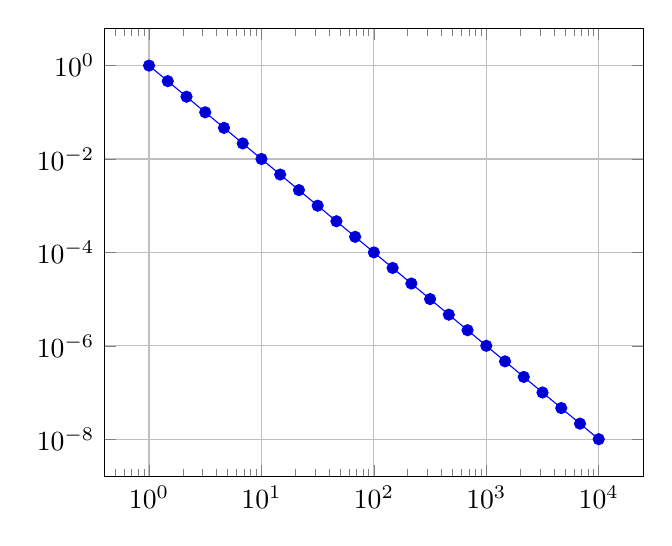
\begin{tikzpicture}
	\begin{loglogaxis}[axis equal image=false,grid=major]
		\addplot expression[domain=1:10000] {x^-2};
	\end{loglogaxis}
\end{tikzpicture}
\hspace{1cm}
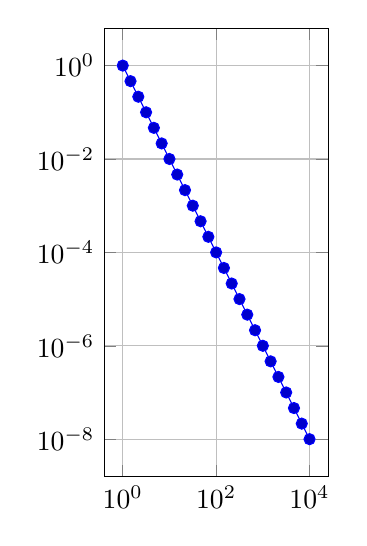
\begin{tikzpicture}
	\begin{loglogaxis}[axis equal image=true,grid=major]
		\addplot expression[domain=1:10000] {x^-2};
	\end{loglogaxis}
\end{tikzpicture}
\end{codeexample}
\end{pgfplotskey}
